The problem of finding every center and angle of rotation of a fixed shape ellipse which makes it have three points on its border is presented in this section. Even though its simple statement--it is short and uses only basic mathematical concepts--we were not able to find any work on it, or even on related problems. 
As a result, starting from scratch, we ended up trying a handful of approaches with most of them failing on the way. We try to give a review of some of those, going through the issues with the failing ones. At the end we propose an algorithm that takes around $6^3$ operations to compute every solution of the problem. Also, we run some experiments to analyze its efficiency in terms of numerical precision and CPU time.

\section{Definition}

We call the problem introduced in this section \sigla{E3PNT}{Ellipse by Three Points}. An instance of it is given by three points $u, v, w \in \R^2$ and the shape parameters of an ellipse $(a, b) \in \R^2_{>0}$, with $a > b$. 

Let $E$ represent the coverage area of an ellipse with the given shape parameters $(a, b)$, then a solution of E3PNT can be defined as a pair $(q, \theta) \in \R^2\times[0, \pi)$, such that $\{u, v, w\} \subset \partial E(q, \theta)$. As a last remark, because of its application on \autoref{chapter:ellipses_n}, a method would only be useful for our case if it can encounter every solution of E3PNT. This requirement, of course, makes the problem more challenging.

\section{Transforming the problem}

Initially, E3PNT is a problem with three unknown variables: the two coordinates of the center point $q_x, q_y, $ and the angle of rotation $\theta$. In this section, we transform E3PNT into the problem of finding the roots of an univariate function using the known problem of determining the circumcircle of a triangle. We also show E3PNT has at most $6$ solutions.

To make the problem simpler, let us translate the system, so the point $u$ is at the origin; that is, assume that the three points given by the E3PNT instance are $(0, 0); v; w$. After that, we assume that the ellipse is actually axis-parallel and the points are the ones rotating. When an angle is found such that the three points lie on the border of the axis-parallel ellipse, a linear transformation can be applied to compress the x-axis by $\frac{b}{a}$ transforming the ellipse into a circle of radius $b$. This transformation can be seen on \autoref{fig:circumscribed-circle} where a solution of the E3PNT is transformed firstly into an axis-parallel ellipse, and then into a circle of radius $b$.
This process can be parameterized by the angle of rotation of the points, as described by

\begin{equation}\label{eq:trpnts}
\varphi(p, \theta)=\left[\begin{array}{cc}
\frac{b}{a}&0\\
0&1
\end{array}\right]
\left[\begin{array}{cc}
\cos{\theta}&\sin{\theta}\\
-\sin{\theta}&\cos{\theta}
\end{array}\right]\left[\begin{array}{c}
p_x\\
p_y
\end{array}\right].
\end{equation}
Also, to make the notation more clear, we denote by $\Lambda(\theta)$ the triangle formed by the points $(0, 0); \varphi(v, \theta); \varphi(w, \theta)$, as long as they are not collinear. This being said, we go further to introduce another problem which is equivalent to E3PNT.

\begin{figure}
	\centering
	\caption{Transforming an ellipse into a circle. T1, T2, and T3 represent the steps of the transformation.}
	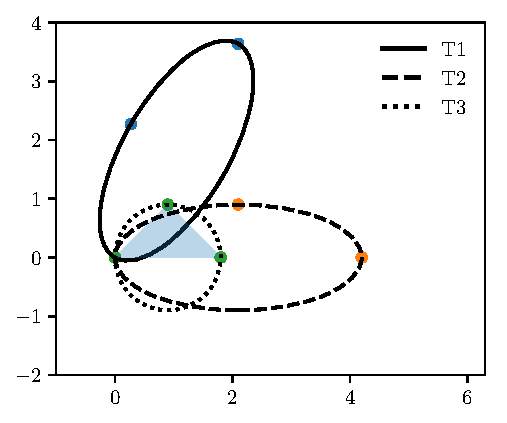
\includegraphics{tex/figures/scripts/circumscribed-circle}
	\fautor
	\label{fig:circumscribed-circle}
\end{figure}

\subsection{A circumradius problem}

The term circumradius, in this work, is used to describe the radius of a triangle's circumscribed circle, which is a circle that has the triangle's vertices on its border. Given an instance of E3PNT, we define the circumradius problem as the problem of determining an angle of rotation $\theta$, such that the circumradius of $\Lambda(\theta)\in[0, \pi)$ is equal to $b$.

As it can be seen on \autoref{fig:circumscribed-circle}, given an instance of E3PNT and an angle of rotation $\theta\in[0, \pi)$ that makes $\Lambda(\theta)$ have a circumradius $b$; a solution for E3PNT can be obtained using the inverse transformation $\varphi^{-1}$. This is possible because for any fixed $\theta$, $\varphi$ is just a linear function which are known to be invertible.
With that in mind, it is possible to conclude that both problems are equivalent because, from a solution of one, an unique solution of the other can be obtained.

The main reason to work with this problem is the reduction in the number of unknown variables from three to just one. This idea, however, would only be useful if checking the existence of a circumscribed circle with radius $b$ is a convenient problem.

It turns out that for three non-collinear points, there is always an unique circumscribed circle. Also, finding this unique circle can be done analytically, and its radius $R$ can be computed through the expression

\begin{equation}\label{eq:circumscribed_circle}
R = \dfrac{\norm{\varphi(v, \theta)}\norm{\varphi(w, \theta)}\norm{\varphi(v, \theta)-\varphi(w, \theta)}   }{4A(\theta)},
\end{equation}
with $A(\theta)$ being the area of the triangle $\Lambda(\theta)$ (for more details about \autoref{eq:circumscribed_circle}, or on how to determine the center of a circumscribed circle see \citeonline[p.~189]{johnson1960}
). It should be pointed out that the transformation does not preserve distance or area; if that was true, the radius defined by \autoref{eq:circumscribed_circle} would be constant.

With the formula for the circumradius in hands, a function can be defined, such that its roots provide solutions for the circumradius problem.
Imposing the radius $R$ to be equal $b$ and squaring to eliminate the square roots present in the Euclidean distance, a function $\xi : [0, 2\pi) \mapsto \mathbb{R}_{>0}$ is defined as 

\begin{equation}\label{eq:circumscribed_circle_b}
\xi(\theta) = 16b^2A(\theta)^2 - \norm{\varphi(v, \theta)}^2\norm{\varphi(w, \theta)}^2\norm{\varphi(v, \theta)-\varphi(w, \theta)}^2.
\end{equation}
Any root of $\xi$ produces a triangle whose circumradius is $b$ and subsequently provides a solution for E3PNT.

The next step is then to develop an algorithm to find every root of $\xi$.
Before continuing with this approach though, it is important to address the question about the number of roots of $\xi$ in the interval $[0, \pi)$.

\subsection{The number of solutions of E3PNT}

One of the steps of the method developed in \autoref{chapter:ellipses_n} is to iterate over every solution of E3PNT for every triplet of points. Of course doing that is only possible for a finite number of solutions. Moreover, even if the number of solutions is finite, discovering a bound for it is essential for determining the algorithm's efficiency.

\begin{lema}
	E3PNT has at most $6$ solutions.
\end{lema}

\begin{proof}
	
Back on \autoref{chapter:definitions}, real trigonometric polynomials were introduced. It was stated that a $n$-degree polynomial can have up to $2n$ distinct roots. It turns out that $\xi$ is a real trigonometric polynomial of degree $6$ and it can be written in the format given by \autoref{eq:trig_poly_2}. This implies that $\xi$ can have up to $12$ distinct roots.
 To show that, just note that it is possible to write $\norm{\varphi(v, \theta)}^2$ and $A(\theta)^2$ in the same form as given by \autoref{eq:trig_poly_2}:
 
 \begin{align}\label{eq:dd}
 	\norm{\varphi(v, \theta)}^2 = (v_x\frac{b}{a}\cos\theta + v_y\frac{b}{a}\sin\theta)^2 + (v_y\cos\theta - v_x\sin\theta)^2\\
 	\label{eq:dd2} A(\theta)^2=\dfrac{1}{4}\det\left(
 	\begin{array}{cc}
 		v_x\frac{b}{a}\cos\theta + v_y\frac{b}{a}\sin\theta&v_y\cos\theta - v_x\sin\theta\\
 		w_x\frac{b}{a}\cos\theta + w_y\frac{b}{a}\sin\theta&w_y\cos\theta - w_x\sin\theta
 	\end{array}\right)^2.
 \end{align}
  It is also possible to see that the term of higher the degree of $\xi$ is the multiplication of the three squared lengths of the triangle formed by the points $\{(0, 0), \varphi(v, \theta), \varphi(w, \theta)\}$. This multiplication has the same degree of $(\norm{\varphi(v, \theta)}^2)^3$, and because $\norm{\varphi(v, \theta)}^2$ has degree $2$, the degree of $\norm{\varphi(v, \theta)}^2$ is $6$ which consequently is the degree of $\xi$.
Going from $12$ solutions to $6$ is done by using the symmetry of ellipses. In \autoref{chapter:definitions}, it was stated that any rotation in the interval $[0, \pi)$ is identical to a rotation in $[\pi, 2\pi)$. Therefore, half of the roots of $\xi$ are in $[\pi, 2\pi)$ and can be dismissed.
\end{proof}

\section{An attempt using the conic general equation}

The idea of this approach was to use the six-parameter conic equation to represent an ellipse. This equation is given by
\begin{equation}\label{eq:gen_ellipse}
Ax^2+Bxy+Cy^2+Dy+Ex+F=0.
\end{equation}
This equation actually represents any conic, for it to be an ellipse the condition $B^2 -4AC < 0$ must be satisfied.

Setting the first point to be the origin, we get $F=0$, using the other two points, it is possible to write $D$ and $E$ in terms of $A, B, C$. As any multiple of \autoref{eq:gen_ellipse} represents the same conic, we can set $B$ to be equal $1$. Then, we end up with two variables, $A$ and $C$, and still need to impose that the final equation represents an ellipse and its major-axis and minor-axis have the predefined value. Let $\Delta=4AC-B^2=4AC-1$, and assume $F=0$, then the expressions for both major-axis and minor-axis respectively are
\begin{align}\label{eq:gen_ellipse_a}
a^2 = \dfrac{2\dfrac{AE^2 -BDE +CD^2}{\Delta}}{A + C - \sqrt{1 + (A-C)^2}}\\
\label{eq:gen_ellipse_b}b^2 = \frac{2\dfrac{AE^2 -BDE +CD^2}{\Delta}}{A + C + \sqrt{1 + (A-C)^2}}.
\end{align}
These two equations define two curves in $\R^2$ with $A$ and $C$ being the chosen variables. The solutions lie in the set of intersection of these curves. Finding this set was judged to be non-trivial and probably could be approximated numerically, however, we decided not to further pursue this approach.

Another idea which has been explored was working with the ratio $\frac{a^2}{b^2}$ which becomes an expression that allows $A$ to be written as a function of $C$. This function appeared, at first we thought, to be monotonic, we tried to develop a method based on that, however, cases where the function does not behave as nicely were found. It is likely that developing a method to approximate solutions working with this function is possible, but we decided not to continue on this track.


\section{An approximation method}

One of the most useful techniques when dealing with complicated functions is approximation. They appear in various methods whenever a derivative or integral needs to be calculated or for example, in our case, when the roots of a function need to be determined. In general, one has a function $f$ that is part of a family of functions $\mathcal{A}$ and wants to select a simpler function $f^*$ from a set of functions $\mathcal{A^*}$, such that $f^*$ is close enough to $f$ \cite[p.~3]{powell}. For this problem, the approximation of $\xi$ on the interval $[0, \pi)$ is considered. The approximation set of functions is going to be the set of $n$-degree Chebyshev polynomials which the roots can be found through determining the eigenvalues of a $n\times n$ matrix.


\subsection{Chebyshev polynomial}

Chebyshev polynomials are widely used in Numerical Analysis in areas like numerical integration, polynomial approximation, and ordinary and partial differential equations.
They are also very useful in practice and are present in extension libraries in Python, MATLAB and C.

Because of the scope of this work, only a brief introduction of Chebyshev polynomials of the first kind and its usage in polynomial interpolation is given. For a more thorough work on the subject, please check the book by \citeonline{chebbook}.

We refer to $T_n : [-1, 1] \mapsto [-1, 1]$ as the $n$-degree Chebyshev polynomial of the first kind, and it is defined as
\begin{equation}
T_n(x) = \cos({n\arccos x}).
\end{equation}
It is important to mention that this definition can be extended to the whole real line. Using some trigonometric identities, $T_n$ can also be expressed as a recurrence relation
\begin{equation}
T_n(x) = 2xT_{n-1}(x) - T_{n-2}(x).
\end{equation}

An important property worth bringing up is that Chebyshev polynomials are orthogonal and form a basis for the polynomial space. This implies that any $p_n$ of degree up to $n$ can be expressed as a truncated Chebyshev series
\begin{equation}\label{eq:chebseries}
p_n(x) = \sum_{j=0}^{n} a_j T_j(x).
\end{equation}

One of the greatest qualities of Chebyshev polynomials is its numerical stability. \citeonline{gautschi:1979} showed that the matrix that maps polynomials onto its coefficients written in the power form\footnote{A polynomial is in the power form or the monomial form if it can be written as $\sum_{j=0}^{n}a_jx^j$.} has a condition number that grows exponentially with $n$. On the other hand, the matrix that converts polynomials to the Chebyshev basis as \autoref{eq:chebseries}, has a linear condition number bounded by $\sqrt{2}n$.

\subsection{Chebyshev interpolation}
Polynomial interpolation is a form of approximating a function by a polynomial of degree $n$ that passes through $n+1$ chosen points. In fact, this polynomial is unique and it is determined by Lagrange's formula
\begin{equation}\label{eq:lagrange}
f_n(x) = \sum_{j=0}^{n} f(x_j)\dfrac{\prod_{k \neq j}^{n+1} (x-x_k)}{\prod_{k \neq j}^{n+1} (x_j-x_k)},
\end{equation}
with $f$ being the function to be approximated, and $f_n$ the unique $n$-degree polynomial that passes through $\{(x_j, f(x_j)): j=0, 1, \dots n\}$. Because of the uniqueness of interpolant polynomials, there is a direct link between the quality of an approximation and the points chosen to interpolate. As a matter of fact, depending on the points one chooses, even increasing the degree of the interpolation makes the approximation worsen. This is known as Runge's phenomenon and an example can be seen in \citeonline[p.~37]{powell} where uniformly spaced points are chosen to interpolate the function $f(x) = (1+x^2)^{-1}$ on the interval $[-5, 5]$. 

That is where Chebyshev interpolation comes in. Instead of choosing $n+1$ arbitrary points, the $n+1$ roots of $T_{n+1}$, which are also known as Chebyshev Nodes, are chosen as the interpolation points. The $n+1$ Chebyshev nodes are given by
\begin{equation}
x_j = \cos{\left(\dfrac{\pi(j-\frac{1}{2})}{n+1}\right)},
\end{equation}
for $j=1, \dots, n+1$. This particular choice defeats Runge's phenomenon and provides a convergent approximation. 
Note that, if the domain of the function to be interpolated is defined on a range other than $[-1, 1]$, let us say $[a, b]$, then the transformation
\begin{equation}
\hat{x_j} = \frac{a+b}{2} + \frac{b-a}{2}x_j
\end{equation}
can be done to map it to the Chebyshev Nodes' domain $[-1, 1]$.

Then, the Chebyshev interpolation of a function $f: [a, b] \mapsto \R$ can be determined using Lagrange's formula and the points $\hat{x}_1, \dots, \hat{x}_n$. 
As it was mentioned in \autoref{chapter:definitions}, finding the roots of a polynomial written in the monomial form can be done by determining the eigenvalues of a so-called Frobenius companion matrix. For small $n$ this works fine, however, converting the polynomial obtained by \autoref{eq:lagrange} to the power form, as $n$ grows, becomes a very ill-conditioned problem. 
An alternative method can be found in \citeonline{boyd:2013} where the Chebyshev interpolation is calculated directly as a truncated Chebyshev series, as in \autoref{eq:chebseries}, in $\bigO(n^2)$. Also, given a polynomial written in the Chebyshev basis, a $n\times n$ matrix can be constructed, such that its eigenvalues are the roots of that polynomial. \citeonline{boyd:2013} refers to this matrix as the Chebyshev-Frobenius companion matrix.

Therefore, the whole process of interpolating and finding the roots can be done using only Chebyshev polynomials, which have great numerical stability. Also, Chebyshev-Frobenius matrices have the same property as companion matrices which allows their eigenvalues to be found by a QR algorithm. Summing the two steps, a $\bigO(n^3)$ algorithm can be achieved, with $n$ being the degree of the interpolation.

The last question that needs to be addressed is how close the roots of the Chebyshev interpolant $f_n$ are to the roots of $\xi$?

Even though $\xi$ is complicated enough, in a sense that finding its roots directly is no trivial task, it is a very well-behaved function: it is analytic and  has infinitely many continuous and integrable derivatives. This satisfy all the requirements of the result in \citeonline[p.~28]{gottlieb} which says that if a function has $m$ continuous and integrable derivatives on a closed interval, then its absolute difference between the Chebyshev truncate series is $\bigO(n^{-m})$. Also, in \citeonline{battles:2004} a theorem is presented stating that if a function is analytic on a neighborhood of $[-1, 1]$, then the convergence is $\bigO(C^n)$, for some $C<1$.

To choose the degree of the interpolation we use the last coefficient rule-of-thumb introduced by \citeonline[p.~50]{boyd:2001}. There is no guarantee that this method will choose $n$, such that $f_n$ is close enough to $\xi$ everywhere on $[0, \pi)$, nonetheless, in practice, it is taken to be a good estimate for the error

\begin{equation}
r_n = \max_{0 \le \theta < \pi} |f_n(\theta) - \xi(\theta)|,
\end{equation}
which measures how far the interpolation is at the point it worst approximates. 

\subsection{Numerical Experiments}

In this section we run some experiments to verify how big the interpolation degree must be for a good precision to be achieved. 
The interpolation was run for several degrees for every triplet of points present in an instance from \citeonline{canbolat}. We considered the error to be $|\xi(\hat{\theta})|$ for every root $\hat{\theta}$ found; simply put we measure how close the roots are to zero.

The results are shown in \autoref{fig:interpolant_error} where the worst error found among every root found is plotted against the interpolant degree used. A parameter $K$ is also used in the experiments. This is an idea suggested in \citeonline{boyd:2013} to improve accuracy, this parameter represents the number of sub-intervals that $[0, \pi)$ is divided into. This way, $K$ interpolations are used to obtain every root in the whole interval. It can be seen in \autoref{fig:interpolant_error} that this strategy helps a lot in improving the accuracy even when not so large degrees are used.

\begin{figure}
	\centering
	\caption{The interpolation error measured on roots that were found.}
	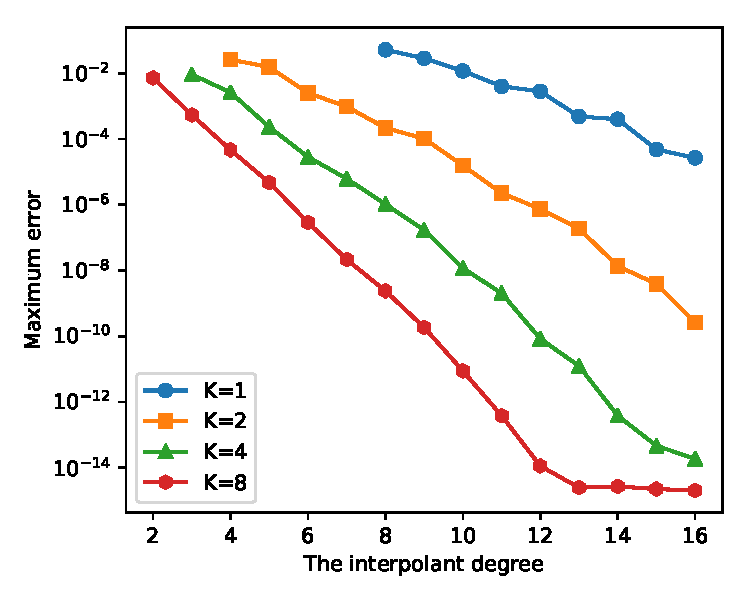
\includegraphics{tex/figures/interpolant_error}
	\fautor
	\label{fig:interpolant_error}
\end{figure}

\section{Converting $\xi$ into a polynomial}

In \autoref{chapter:definitions}, a brief introduction is given on how to get the roots of a polynomial. For that reason, we discuss two ways of converting $\xi$ into a polynomial in this section. Symbolic computing was used to compute the polynomials, the Python external library called SymPy was utilized (see \citeonline{sympy} for more details).

\subsection{Real polynomial}

The first attempt was using the identity $x = \tan{\frac{\theta}{2}}$ from which it is possible to construct a $12$-degree polynomial. At first,  the root-finding algorithm described on \autoref{chapter:definitions} seemed to work fine and return every solution of E3PNT, however, we later found out that for some instances, priorly known roots were not being found. The cause was not for sure identified, but a good guess would be that for angles which are greater than $\frac{\pi}{4}$, $x$ starts growing too rapidly which could lead to numerical instability. This issue made us abandon this approach and pursue a different way to convert $\xi$ into a polynomial.

\subsection{Complex polynomial}

The second approach is based on a idea published in \citeonline{boyd:2006} which uses the identities on \autoref{eq:complex_trig} to convert real trigonometric polynomials, which is the case of $\xi$, into univariate complex polynomials. This approach is preferable as it preserves the numerical stability of the original real trigonometric polynomial--more details about this can be found in \citeonline{weidner} where it is said that computing the roots of a real trigonometric polynomial through this transformation does not yield loss of accuracy.

\begin{align}\label{eq:complex_trig}
\cos{\theta} = \dfrac{e^{i\theta} + e^{-i\theta}}{2}\\
\sin{\theta} = \dfrac{e^{i\theta} - e^{-i\theta}}{2i}.
\end{align}

It is possible to show that with that substitution and changing the variable to $z=e^{i\theta}$, we obtain the following function $g : \mathbb{S} \mapsto \mathbb{C}$, with $\mathbb{S}$ being the unit complex circle ($\mathbb{S} = \{z \in \mathbb{C} : |z|=1\}$):

\begin{equation}
g(z)=\sum_{k=0}^{12} c_k z^{k-6},
\end{equation}
for some $c_0, \dots, c_{12} \in \mathbb{C}$. As the equalities on \autoref{eq:complex_trig} are valid for any $\theta \in \R$, the function $g(e^{i\theta})$ and the function $\xi$ are equivalent since $g(e^{i\theta}) = \xi(\theta)$ for any $\theta \in [0, 2\pi)$. 

The function $g$ is still not a polynomial as $z$ shows up with negative exponents (up to $-6$), and its domain is the unit circle $\mathbb{S}$, not the whole complex set $\mathbb{C}$. 
The first issue can be fixed by multiplying $g$ by $z^6$, note that this does not create further problems as $0\not\in \mathbb{S}$. The second issue is removed by simply extending the domain from $\mathbb{S}$ to $\mathbb{C}$, as $\mathbb{S} \subset \mathbb{C}$, roots outside the unit circle could appear which requires a further check for every root that is found.
Finally, from $g$, the polynomial $h : \mathbb{C} \mapsto \mathbb{C}$ is defined as

\begin{equation}\label{eq:h}
h(z) = z^6 g(z) = \sum_{k=0}^{12} c_k z^k.
\end{equation}
By its definition it is possible to see that every root of $g$ is also a root of $h$, and conversely, every root of $h$ which is in $\mathbb{S}$, is also a root of $g$. Lastly, every root of $g$ will correspond to a root of $\xi$ through their angles on the unit circle.

\subsubsection{Further improvements}

It is possible to make another reduction to obtain a degree-$6$ polynomial.
As it has been mentioned before, an ellipse is symmetric with respect to its own major or minor axis. 
In other words, rotating an ellipse by $\theta \in [0, \pi)$ is the same as rotating the same ellipse by $\pi + \theta$.
On the other hand, in \autoref{chapter:definitions}, it was stated that the angle of the complex numbers $z$ and $-z$ has the same symmetry with each other as the aforementioned symmetry of ellipses:
\begin{equation*}
angle(-z) = \pi + angle(z).
\end{equation*}
From that, as $g(e^{i\theta})=\xi(\theta)$ for every $\theta \in [0, 2\pi)$, we conclude that $g(-z)=g(z)$. This implies that $h$ is, in fact, an even polynomial, or that $h(-z) = h(z)$ is true for every $z\in\mathbb{C}$:
\begin{align}
h(-z) = (-z)^6g(-z) = z^6g(z).
\end{align}
Therefore, all the odd degree coefficients of $h$ are zero and we can define the $6$-degree polynomial $f : \mathbb{C} \mapsto \mathbb{C}$ with the substitution $y=z^2$ as follows
\begin{equation}
f(y) = \sum_{k=0}^{6} c_{2k} y^k.
\end{equation}
Then from every root $\hat{y}$ of $f$, two roots of $h$ can be obtained: $\sqrt{\hat{y}}$ and $-\sqrt{\hat{y}}$. As the angle of one of the roots will not be between $[0, \pi)$ we can ignore one of them. 
Note that the the square root of $\hat{y}$ does not need to be calculated, as only the angles are needed and they can be obtained by the identity
\begin{equation}
angle(\sqrt{z}) = angle(z)/2.
\end{equation}

It is also worth mentioning that a pattern on the coefficients of $f$ was identified, and maybe, for future work, it can be used for further improvements. Analyzing the polynomials produced for several instances, the following seems to be true:
\begin{equation}\label{eq:palindromic_pol}
c_k = \overline{c_{6-k}},
\end{equation}
for $k=0, \dots, 6$. For now, we neither have any ideas on how \autoref{eq:palindromic_pol} could be proved nor how it could be used to find the roots of $f$.

Finally, in the next section we use this approach of converting $\xi$ into a complex polynomial to develop an algorithm for E3PNT.

\section{An algorithm for E3PNT}

Among the approaches that have been described here, converting $\xi$ into a complex polynomial was the chosen one as the basis of the algorithm for E3PNT.
The other approach that showed good results was the numerical approximation one that uses Chebyshev interpolation. Ultimately this approach requires finding the eigenvalues of a companion matrix, this matrix, however, is usually going to be larger than the $6\times 6$, which is the size of the matrix needed to find the roots of the complex polynomial in \autoref{algoritmo:e3p}. 

Details about getting the eigenvalues of a companion matrix, or determining the center of a circumscribed circle of a triangle are omitted from \autoref{algoritmo:e3p} for the sake of clarity and can be found elsewhere in this work. Also, we assume that the $angle$ function used in the algorithm returns the angle of a complex number in the interval $[0, 2\pi)$.


\begin{algoritmo}
	\caption{The algorithm for E3P.}\label{algoritmo:e3p}
	\begin{algorithmic}[1]
		\Require{$u, v, w\in\R^2$, and $a, b\in\R_{>0}$, with $a>b$.}
		\Ensure{Every solution of E3P.}
		
		\item[]
		
		\Procedure{$E3PNT$}{$u,v,w,a,b$}
		
		\State $\hat{u}\gets (0,0)$
		\State $\hat{v} \gets v-u$
		\State $\hat{w} \gets w-u$
		
		\State Let $c_0, \dots, c_{12}$ be the coefficients of polynomial $h$ as \autoref{eq:h}.
		\State Let $A$ be a $6\times6$ zero matrix.
		
		\For{$i\in\{1, \dots, 6\}$}\Comment{Constructing the companion matrix.}
			\State $A_{i,i+1} \gets 1$
			\State $A_{6,i} \gets -\dfrac{c_{2(i-1)}}{c_{12}}$
		\EndFor

		
		\State $Q \gets \{\}$
		
		\ForAll{$q \in eig(A)$} \Comment{$eig(A)$ returns every eigenvalue of $A$.}
		\State $\theta\gets \min\{angle(-q)/2, angle(q)/2\}$
		\If{$|\theta|=1$}
			\State Let $c$ be the center of the circumscribe circle of $\Lambda(\theta)$.
			\State $Q \gets Q\cup \{(\varphi^{-1}(c, \theta)+u, \theta)\}$
		\EndIf
		\EndFor
				
		\State \Return $Q$
		\EndProcedure
	\end{algorithmic}
\end{algoritmo}

\begin{teorema}
	The \autoref{algoritmo:e3p} computes every solution of E3PNT in $\bigO(1)$ operations.
\end{teorema}

\begin{proof}
	It has already been shown that computing every root of $\xi$ through the complex polynomial yields every solution of E3PNT, the only thing left to prove is the running time of the algorithm.
	Computing every eigenvalue of a matrix can be done in $\bigO(n^3)$, but as for our case $n$ is fixed at $6$, it can be stated that computing the eigenvalues for the companion matrix of $f$ can be done in $\bigO(1)$. Therefore, the whole algorithm runs in constant time.
\end{proof}

\subsection{Numerical Experiments}

In this section we show the results of an experiment made to study the numerical stability of \autoref{algoritmo:e3p}.
For every root found $\hat{\theta}$, we measure its error by $|\xi(\hat{\theta})$|.

We generate random instances according to a normal distribution with $0$ mean and standard deviation $K$. We tried different values for $K$ and generated $1000$ instances for each one. The maximum error and the average error for different values of $K$ can be seen in \autoref{fig:e3p_error}.

From this experiment we can say that \autoref{algoritmo:e3p} has a good numerical stability as the accuracy of the roots found shows to have a linear relation .

\begin{figure}
	\centering
	\caption{The interpolation error measured on roots that were found.}
	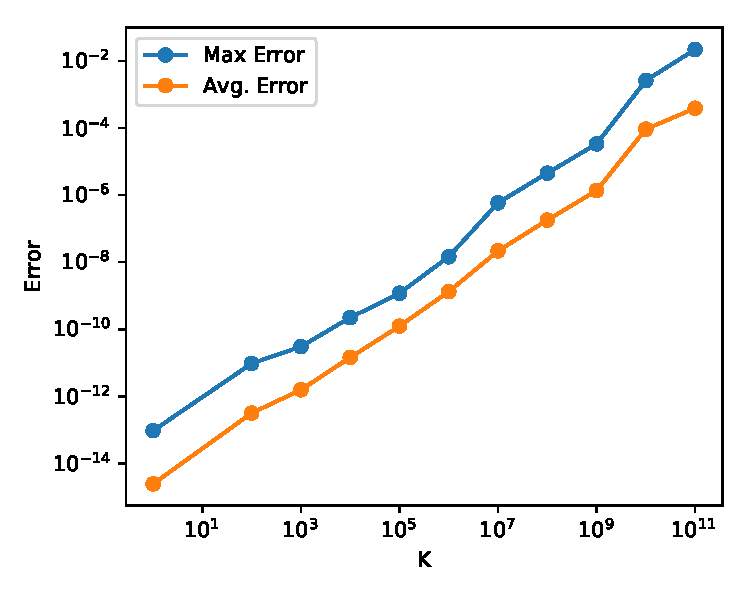
\includegraphics{tex/figures/e3p_error}
	\fautor
	\label{fig:e3p_error}
\end{figure}